\section{Jet Algorithms}

Final states containing coloured partons undergo parton showering and hadronisation as outlined in section \ref{eventgenerators}. This means  that the observable final state will consist of collimated streams of hadrons, which are called jets. Naively, one would expect a di-parton system to result in a two-jet final state. However, hard, wide-angle gluon radiation can occur in the parton showering stage and this would produce a new stream of particles and could look like a three-jet system. The exact classification of a system in terms of the number of jets depends on the jet algorithm used. In this section, the mid-point cone and $K_T$ clustering jet algorithms are reviewed.
%should I state what a jet algorithm should do...ideal.

The ideal jet algorithm, as defined by a Tevatron Run II Jet Physics working group \cite{Blazey:2000qt}, should possess the following criteria:
\begin{enumerate}
\item The algorithm should be fully defined.
\item The algorithm should be collinear and infrared safe.
\item It should perform equally well at parton, hadron and detector level.
\item It should not depend on detector quantities such as cell or tower size.
\end{enumerate}
The last two criteria will only ever be approximately true in a real algorithm due to detector resolution and granularity. The size of the towers and cells will never allow the direction of the particle to be exactly known, hence the algorithm will perform slightly differently at detector level. The first criterion is a requirement of the algorithm definition. The second criterion is required so that not only is the perturbative QCD calculation free of soft and collinear singularities, but the result after jet-finding is insensitive to soft or collinear radiation.

\subsection{The Mid-Point Cone Algorithm}

The mid-point cone algorithm has a geometrical motivation and defines a jet to be a group of particles within a cone of radius, $R_{cone}$, in $\eta \times \phi$ space. The cone radius is used to define the spatial extent of the jet. The basic cone algorithm \cite{Blazey:2000qt} works as follows:
\begin{enumerate}
\item A seed is assigned to every particle or calorimeter tower. This seed is used as the centroid direction, $\left(\eta^C, \phi^C\right)$, for a proto-jet. 

\item All particles, $i$, that satisfy the requirement
\begin{equation}
\left( \eta^i - \eta^C \right)^2 + \left( \phi^i -\phi^C \right)^2 \leq R_{cone}^2
\end{equation}
are then clustered to find the proto-jet. The axis of the proto-jet, $\left(\eta^J, \phi^J\right)$, is found by the $E_T$ weighted sum of particles in the jet, i.e
\begin{equation}
\eta^J = \frac{\sum{E_T^i\eta^i}}{\sum{E_T^i}} \quad \text{and} \quad
\phi^J = \frac{\sum{E_T^i\phi^i}}{\sum{E_T^i}}
\end{equation}
where the sum is over all particles within the cone, $C$.

\item The proto-jet axis is then used as the seed for a new cone and step 2 repeated. In this way, the calculation is iterated to find stable proto-jets when $\eta^C = \eta^J$ and $\phi^C = \phi^J$.

\item Steps 2 and 3 are repeated to find all possible proto-jets.

\item The above procedure produces jets which overlap in $\eta \times \phi$ space. In this case, the lower transverse energy jet is discarded if the fraction, $f$, of its energy that is shared with the other jet is greater than an overlap fraction, $O$. If $f < O$, then the particles in the overlap region are assigned to the nearest jet centre.

\end{enumerate}

This algorithm would not be infra-red safe as it stands. Figure \ref{infraredcone} highlights the problem of soft radiation in the middle of two possible proto-jets which are separated by more than $R_{cone}$ in $\eta \times \phi$ space, but less than $2R_{cone}$. It is clear that the number of jets in the final state is dependent on whether soft radiation is emitted between the jets. In the absence of the soft radiation, two jets would be found. However, the soft radiation between the jets would provide a new seed and only one jet would be found. Hence the final result is sensitive to soft radiation between the jets. 


\begin{figure}[t]
\centering
	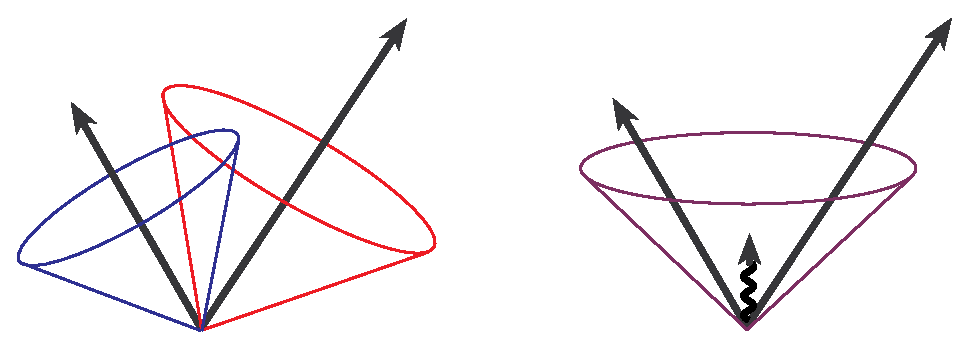
\includegraphics[width=0.8\textwidth]{Diagrams/cone-fig1.eps}
\caption[Infra-red sensitivity of a basic cone algorithm]{Infra-red sensitivity of a basic cone algorithm \cite{Blazey:2000qt}. The two hard partons, represented as arrows, are separated by more than $R_{cone}$ but less than $2R_{cone}$. In the absence of radiation between the jets (left), 2 distinct jets will be found. However, radiation between the jets (right) would cause only 1 jet to be found. \label{infraredcone}}
\end{figure}

This problem is removed if, in addition to using the particles as seeds, a seed is created in the middle (in $\eta \times \phi$) of every two particles that are separated by less than $2R_{cone}$. Now the final result is independent of soft radiation. This type of algorithm is called a mid-point cone algorithm.

\subsection{The $K_T$ Clustering Algorithm}

The $K_T$ algorithm is kinematically motivated. The prescription is to merge particles together if they have a low transverse momentum with respect to one another. The basic inclusive $K_T$ algorithm, outlined in \cite{Butterworth:2002xg}, defines jets in the following way:

\begin{enumerate}

\item The resolution variables, $d_{kB}$ and $d_{kl}$, are computed for every object, $k$, and every pair of objects, $k$ and $l$. The resolution variables are defined to be
\begin{equation*}
d_{kB} = p_{Tk}^2 \qquad \text{and}
\end{equation*}
\begin{equation}
d_{kl} = \text{min}\left(p_{Tk}^2, p_{Tl}^2\right)\left[\left(\eta_k - \eta_l\right)^2 + \left(\phi_k - \phi_l\right)^2\right]  \, .
\end{equation}
At the start of the algorithm, the list of objects are particles or calorimeter towers.

\item The $d_{kB}$ are scaled by 
\begin{equation}
d_k = R_{K_T}^2 d_{kB}
\end{equation}
where $R_{K_T}$ is a user defined parameter.

\item The smallest resolution variable is found in the set of $d_k$ and $d_{kl}$. If this is one of the  $d_{kl}$, then objects $k$ and $l$ are merged into a single object. If one of the $d_k$ is the smallest resolution variable then $k$ is defined as a jet and removed from the list.

\item Steps 1 - 3 are repeated until all objects are defined as jets.

\end{enumerate}
This algorithm is insensitive to soft or collinear radiation. It is the nature of the $K_T$ algorithm to merge soft/collinear particles first because these have the smallest $d_{kl}$ resolution variable. 



